\documentclass[12pt,a4paper,twoside,headsepline,parskip=half]{scrreprt}

% ---------- Seitenlayout ----------
\usepackage[
    a4paper,
    twoside,
    left=3cm,       % Innenrand (Bindung)
    right=2.5cm,    % Außenrand
    top=2.5cm,
    bottom=2.5cm,
]{geometry}

% ---------- Sprache & Kodierung ----------
%\usepackage[T1]{fontenc}
\usepackage{fontspec}
\usepackage[ngerman]{babel}

% ---------- Zeilenabstand ----------
\usepackage{setspace}
\onehalfspacing

% ---------- Schrift ----------
\usepackage{lmodern}

% ---------- Mathematik & Symbole ----------
\usepackage{amssymb}
\usepackage{amsmath}
\usepackage{siunitx}

% ---------- Listen & Absätze ----------
\usepackage{enumitem}

% ---------- Tabellen, Grafiken, Gleitobjekte ----------
\usepackage{graphicx}
\usepackage{tikz}
\usetikzlibrary{positioning}
\usepackage{svg}
\usepackage{xltabular}
\usepackage{tabularx}
\usepackage{booktabs}
\usepackage{caption}
\usepackage{float}
\usepackage{pdflscape}

% ---------- Verbatim / Zitate ----------
\usepackage{verbatim}
\usepackage{csquotes}

% ---------- Literaturverzeichnis ----------
\usepackage[backend=biber, style=ieee, sortcites=true]{biblatex}
\addbibresource{literatur.bib}

% ---------- Hyperlinks (immer nach den meisten anderen Paketen laden) ----------
% Bessere Umbrüche: Randausgleich und Dehnung, damit lange \texttt{}-Bezeichner
% (z. B. gtest\_discover\_tests) nicht in den Rand laufen.
\usepackage{microtype}
\setlength{\emergencystretch}{3em}

\usepackage[colorlinks=true,linkcolor=blue,citecolor=blue,urlcolor=blue]{hyperref}

% Seiten auf natuerlicher Hoehe enden lassen, statt den Rest auf die
% Absatzabstaende zu verteilen (sichtbar bei Seiten vor grossen Gleitobjekten).
\raggedbottom

\begin{document}

% ============ TITELSEITE ============
\begin{titlepage}
\centering


\includegraphics[width=0.28\textwidth]{img/06_Matjpg.png}\par
\vspace{0.8cm}

{\large\scshape Universität Potsdam\par}
\vspace{2mm}
{\normalsize Mathematisch-Naturwissenschaftliche Fakultät\par}
{\normalsize Institut für Informatik \& Computational Science\par}

\vfill

{\Large\scshape Bachelorarbeit\par}
\vspace{6mm}

\rule{0.6\textwidth}{0.4pt}\par
\vspace{6mm}

{\LARGE\bfseries Konzeption und Implementierung eines
AST-basierten Frameworks \\ zur Identifizierung
und Analyse \\ von Test-Artefakten in C++
und CMake Forschungs-Repositories\par}

\vspace{6mm}
\rule{0.6\textwidth}{0.4pt}\par

\vfill

\begin{tabular}{@{}ll@{\hspace{3mm}}l@{}}
\textbf{Gutachter:innen:} & Dr.~Mario Frank & (1.\ Gutachten) \\
 & Prof.~Dr.~Anna-Lena Lamprecht & (2.\ Gutachten) \\[6mm]
\textbf{Autor:} & Oskar Soth (806965) &
\end{tabular}

\vspace{1.2cm}
{\large \today\par}

\end{titlepage}

% ============ VORSPANN ============
\pagenumbering{roman}

% Abstract / Kurzfassung
\chapter*{Abstract}
\thispagestyle{empty}
% TODO: English abstract here

\tableofcontents


\clearpage
\pagenumbering{arabic}

\chapter{Einleitung}
\chapter{Grundlagen}
\chapter{Stand der Technik}
\chapter{Anforderungsanalyse und Methodik}
\chapter{Implementierung}
%%%%%%%%%%%%%%%%%%%%%%%%%%%%%%%%%%%%%%%%%%
%%%%%%%%%%%% Implementierung %%%%%%%%%%%%%
%%%%%%%%%%%%%%%%%%%%%%%%%%%%%%%%%%%%%%%%%%

\section{Überblick und Architektur}
\label{sec:impl-ueberblick}

Den Ausgangspunkt der Implementierung bildet das im SWORDS-Projekt entwickelte
textbasierte Analysewerkzeug \cite{SWORDS_template_UP_2024}. Dessen Aufgabenstellung
wird unverändert übernommen: Für eine gegebene Menge von Forschungs-Repositories soll
bestimmt werden, ob und in welcher Form sie Test-Artefakte enthalten. Verändert wird
allein das Verfahren, mit dem diese Bestimmung erfolgt: An die Stelle regulärer
Ausdrücke tritt eine Analyse auf dem Syntaxbaum. Diese bewusste Beschränkung auf eine
einzige veränderte Variable ist Voraussetzung dafür, dass die spätere Evaluation
(Kapitel~\ref{chap:evaluation}) beobachtete Unterschiede dem Analyseverfahren
zurechnen kann und nicht einer gleichzeitig veränderten Aufgabenstellung.

\paragraph{Ein- und Ausgabe.}
Das Werkzeug erhält eine CSV-Datei mit Repository-Metadaten, klont die dort
verzeichneten Repositories und analysiert deren Build-Dateien. Es erzeugt zwei
Ausgaben: eine CSV-Datei mit aggregierten Kennzahlen je Repository, die der
unmittelbaren Vergleichbarkeit mit dem Referenzwerkzeug dient, sowie ein
strukturiertes Testinventar im JSON-Lines-Format, das die rekonstruierten
Testregistrierungen einzeln ausweist. Die Trennung beider Ausgaben wird in
Abschnitt~\ref{sec:impl-ergebnis} begründet.

\paragraph{Zweiteilung des Analyseverfahrens.}
Die zentrale Entwurfsentscheidung der Implementierung ist die Aufteilung der Analyse
in zwei aufeinander aufbauende Durchläufe.

Der \emph{syntaktische Durchlauf} arbeitet dateilokal. Er überführt jede CMake-Datei
mithilfe von Tree-sitter \cite{treesitter} in einen Syntaxbaum und extrahiert daraus
die syntaktischen Bestandteile: Kommandoaufrufe, Makro- und Funktionsdefinitionen,
Schleifen sowie Bedingungsblöcke. Dieser Durchlauf ersetzt die lexikalische Analyse
des Referenzwerkzeugs und ist funktional mit ihr vergleichbar.

Der \emph{semantische Durchlauf} arbeitet über das gesamte Repository. Er bildet das
Auswertungsmodell von CMake nach, indem er bestimmt, welche Dateien überhaupt
ausgewertet werden, Makroaufrufe mit gebundenen Argumenten expandiert und die so
rekonstruierten Testregistrierungen mit den Zielen und Quelldateien verknüpft, auf die
sie sich beziehen.

Die Notwendigkeit dieser Trennung ergibt sich aus einer Eigenschaft des
Untersuchungsgegenstands: Ob eine in einer Datei gefundene Makrodefinition überhaupt
zur Ausführung gelangt, lässt sich aus dieser Datei allein nicht entscheiden, da der
Aufruf in einer beliebigen anderen Datei des Projekts stehen kann. Ein rein
dateilokales Verfahren kann eine Definition folglich nicht von einer Aufrufstelle
unterscheiden, und das gilt für jedes zeilenweise arbeitende textbasierte Verfahren
gleichermaßen.
Erst die auf das gesamte Repository erweiterte Sicht des zweiten Durchlaufs macht diese Unterscheidung
möglich. Sie ist die Grundlage sämtlicher in Abschnitt~\ref{sec:impl-semantisch}
beschriebener Analyseschritte.

% Quelle der Abbildung: diagramme/ablauf_pipeline.puml
% Neu rendern: java -jar plantuml.jar -tpdf diagramme/ablauf_pipeline.puml
\begin{figure}[H]
    \centering
    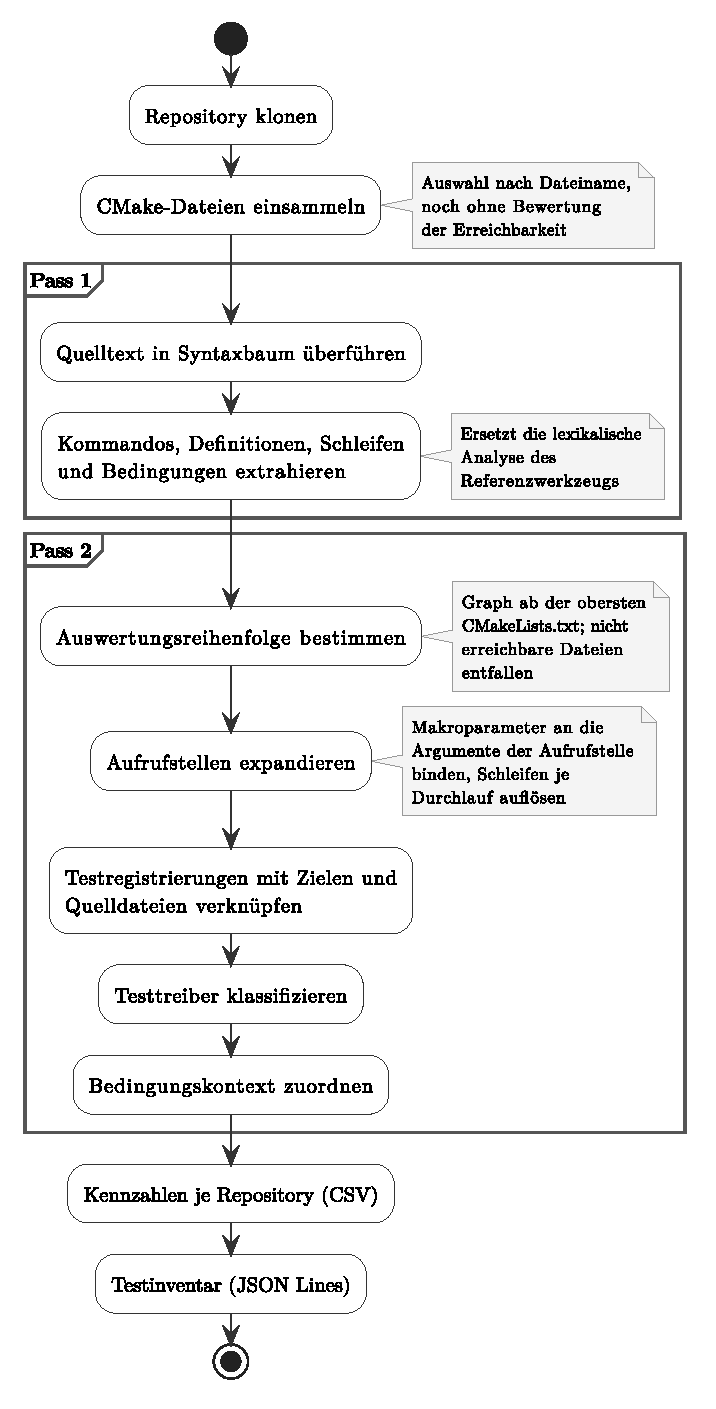
\includegraphics[height=0.62\textheight]{diagramme/ablauf_pipeline.pdf}
    \captionsetup{width=0.9\linewidth}
    \caption{Ablauf der Analyse. Pass~1 ist der syntaktische Durchlauf und
    verarbeitet jede Datei einzeln; Pass~2 ist der semantische Durchlauf und wertet
    das Repository als Ganzes aus.}
    \label{fig:impl-ablauf}
\end{figure}

\paragraph{Modulstruktur.}
Die Implementierung ist in neun Module gegliedert, deren Abhängigkeiten
zyklenfrei geschichtet sind (Tabelle~\ref{tab:impl-module}). Die unterste Schicht
enthält ausschließlich technische Grundlagen ohne fachlichen Bezug; darauf setzt das
Datenmodell auf, darüber die Extraktions- und Analysemodule, und erst das
orchestrierende Modul \texttt{cmake\_parser} kennt alle übrigen. Die Anbindung an
Tree-sitter ist vollständig in \texttt{tree\_sitter\_backend} gekapselt, sodass eine
zusätzliche Sprache durch Ergänzung eines Extraktions- und eines Ergebnismoduls
eingebunden werden kann, ohne die Analyselogik zu verändern. Damit erfüllt die
Architektur die in Abschnitt~\ref{sec:nicht-funktionale-anforderungen} formulierte
Anforderung an die Modularität; Abschnitt~\ref{sec:eval-erweiterbarkeit} greift diesen
Punkt für die Bewertung der Erweiterbarkeit wieder auf.

\begin{table}[H]
    \centering
    \small
    \begin{tabularx}{\textwidth}{l l X}
        \toprule
        \textbf{Schicht} & \textbf{Modul} & \textbf{Aufgabe} \\
        \midrule
        0 & \texttt{common}              & Gemeinsame Datentypen und Hilfsfunktionen \\
        0 & \texttt{tree\_sitter\_backend} & Parserbau, Query-Verwaltung, Quelltextzugriff \\
        1 & \texttt{cmake\_results}      & Datenmodell der Analyseergebnisse \\
        2 & \texttt{source\_collector}   & Auffinden der zu analysierenden Dateien \\
        2 & \texttt{cmake\_ast}          & Extraktion der Syntaxbestandteile \\
        2 & \texttt{cmake\_graph}        & Auswertungsreihenfolge und Erreichbarkeit \\
        2 & \texttt{cmake\_semantics}    & Expansion, Bindung und Klassifikation \\
        2 & \texttt{inventory}           & Serialisierung des Testinventars \\
        3 & \texttt{cmake\_parser}       & Orchestrierung beider Durchläufe \\
        \bottomrule
    \end{tabularx}
    \caption{Module der Implementierung. Module einer Schicht greifen ausschließlich
    auf tiefere Schichten zu.}
    \label{tab:impl-module}
\end{table}

\paragraph{Aufbau des Kapitels.}
Abschnitt~\ref{sec:impl-syntaktisch} beschreibt den syntaktischen Durchlauf und die
Maßnahmen, mit denen dessen Heuristik an die des Referenzwerkzeugs angeglichen wurde.
Abschnitt~\ref{sec:impl-semantisch} stellt den semantischen Durchlauf dar, der den
eigentlichen Beitrag dieser Arbeit bildet.
Abschnitt~\ref{sec:impl-ergebnis} behandelt die Ergebnisrepräsentation,
Abschnitt~\ref{sec:impl-qualitaet} die Maßnahmen zur Qualitätssicherung.
Abschnitt~\ref{sec:impl-grenzen} benennt abschließend die Grenzen der Implementierung.

\section{Syntaktische Ebene}
\label{sec:impl-syntaktisch}

Der syntaktische Durchlauf ersetzt die lexikalische Analyse des Referenzwerkzeugs,
ohne dessen Prüfbedingungen zu verändern. Er beantwortet dieselben Fragen anhand
derselben CMake-Kommandos, leitet die Antwort jedoch aus der Struktur des Syntaxbaums
statt aus dem Zeilentext ab. Dieser Abschnitt beschreibt zunächst die Anbindung an die
Grammatik und die verwendete Query-Sprache, anschließend die extrahierten
Syntaxbestandteile und schließlich die Angleichung der Heuristik an das
Referenzwerkzeug, die den späteren Vergleich beider Verfahren erst aussagekräftig
macht.

\subsection{Grammatik-Anbindung und Query-Sprache}
\label{sec:impl-grammatik}

\paragraph{Parserbau.}
Tree-sitter trennt den Parsergenerator von den Grammatiken, sodass jede Sprache als
eigenständiges Paket eingebunden wird \cite{treesitter}. Die Implementierung nutzt die
Grammatiken \texttt{tree-sitter-cmake} und \texttt{tree-sitter-cpp}. Der gesamte
Zugriff auf die Bibliothek ist im Modul \texttt{tree\_sitter\_backend} gekapselt, das
den Parserbau, das Einlesen der Quelldateien und die Verwaltung der Queries
übernimmt. Kompilierte Queries werden dabei je Kombination aus Sprache und
Query-Quelltext zwischengespeichert, da dieselbe Query über alle zu analysierenden
Dateien hinweg unverändert wiederverwendet wird.

\paragraph{Konkreter und abstrakter Syntaxbaum.}
Tree-sitter erzeugt einen \emph{konkreten} Syntaxbaum (Concrete Syntax Tree, CST),
der den Quelltext lückenlos abdeckt und damit auch Klammern, Trennzeichen und
Kommentare als Knoten enthält. Ein \emph{abstrakter} Syntaxbaum (Abstract Syntax
Tree, AST) im Sinne des Compilerbaus enthält demgegenüber nur die bedeutungstragenden
Knoten \cite{Aho_Lam_Sethi_Ullman_2007}. Tree-sitter bildet diesen Unterschied nicht
durch zwei getrennte Bäume ab, sondern durch die Unterscheidung zwischen benannten und
unbenannten Knoten (\emph{named} und \emph{unnamed nodes}): Knoten, die in der
Grammatik einer benannten Regel entsprechen, tragen den Regelnamen, während wörtliche
Bestandteile wie
die Klammern eines Kommandoaufrufs unbenannt bleiben. Die Query-Sprache adressiert
ausschließlich benannte Knoten und liefert damit genau die Sicht, die in der
Terminologie des Compilerbaus dem abstrakten Syntaxbaum entspricht. Die vorliegende
Arbeit verwendet die Bezeichnung \enquote{AST-basiert} in diesem Sinne: Zugrunde liegt
ein konkreter Syntaxbaum, ausgewertet wird jedoch ausschließlich dessen abstrakte
Sicht.

\paragraph{Query-Sprache.}
Queries werden als S-Expressions formuliert, die ein Teilmuster des Baums beschreiben.
Knotentypen stehen in Klammern, Verschachtelung im Muster entspricht der
Eltern-Kind-Beziehung im Baum. Einem Knoten kann mit dem Präfix \texttt{@} ein
\emph{Capture} zugeordnet werden, unter dem die getroffenen Knoten im Ergebnis
abrufbar sind. Quantoren geben an, wie oft ein Teilmuster auftreten darf:
\texttt{*} für beliebig oft und \texttt{?} für optional.
Abbildung~\ref{fig:impl-query} stellt Quelltext, Syntaxbaum und Query an einem
Beispiel gegenüber.

\begin{figure}[H]
    \centering
    \footnotesize

    \textbf{(a) Quelltext}\\[2pt]
    \texttt{add\_test(NAME smoke COMMAND demo)}\\[10pt]

    \textbf{(b) Syntaxbaum (benannte Knoten)}\\[4pt]
    \begin{tikzpicture}[
        every node/.style={font=\scriptsize},
        knoten/.style={draw=black!55, rounded corners=2pt, inner sep=3pt,
                       font=\scriptsize\ttfamily, align=center},
        treffer/.style={knoten, fill=blue!10, draw=blue!65, thick},
        argument/.style={knoten, fill=orange!14, draw=orange!75, thick, dashed},
        kante/.style={draw=black!55}
    ]
        \node[knoten] (sf)  at (5.2,  0.0) {source\_file};
        \node[knoten] (nc)  at (5.2, -1.0) {normal\_command};
        \node[treffer](id)  at (1.9, -2.1) {identifier\\add\_test};
        \node[knoten] (al)  at (8.5, -2.1) {argument\_list};
        \node[argument](a1) at (4.6, -3.4) {argument\\NAME};
        \node[argument](a2) at (7.2, -3.4) {argument\\smoke};
        \node[argument](a3) at (9.8, -3.4) {argument\\COMMAND};
        \node[argument](a4) at (12.4,-3.4) {argument\\demo};

        \draw[kante] (sf) -- (nc);
        \draw[kante] (nc) -- (id);
        \draw[kante] (nc) -- (al);
        \foreach \a in {a1,a2,a3,a4} \draw[kante] (al) -- (\a);
    \end{tikzpicture}\\[10pt]

    \textbf{(c) Query}\\[4pt]
    \begin{tabular}{@{}l@{}}
        \texttt{(normal\_command} \\
        \hspace*{1.2em}\texttt{(identifier)} \colorbox{blue!10}{\texttt{@command.name}} \\
        \hspace*{1.2em}\texttt{(argument\_list (argument)*}
            \colorbox{orange!14}{\texttt{@command.arg}}\texttt{)?)} \\
    \end{tabular}

    \captionsetup{width=0.92\linewidth}
    \caption{Quelltext, zugehöriger Syntaxbaum und die darauf passende Query. Die
    Einfärbung ordnet die beiden Captures der Query den Knoten zu, die sie
    treffen. Der Quantor \texttt{*} bindet alle Argumente an dasselbe Capture, der
    Quantor \texttt{?} lässt die \texttt{argument\_list} insgesamt entfallen.}
    \label{fig:impl-query}
\end{figure}

\paragraph{Begründung der Query-Sprache.}
Die Alternative zur Query-Sprache ist ein manueller Durchlauf des Baums, bei dem für
jeden Knoten dessen Typ geprüft wird. Ein früherer Entwicklungsstand der vorliegenden
Implementierung ging so vor und erkannte Kommandoaufrufe daran, dass der Knotentyp die
Substring \texttt{command} enthält. Diese Bedingung trifft in der verwendeten
CMake-Grammatik jedoch auf 20 verschiedene Knotentypen zu, darunter
\texttt{if\_command}, \texttt{endif\_command} und \texttt{macro\_command}. Der
Prüfschritt stützte sich damit auf die Schreibweise von Knotennamen und nicht auf die
Struktur des Baums.

Die Query-Sprache beschreibt die gesuchte Struktur stattdessen deklarativ und prüft
sie gegen die Grammatik. Ein Muster, das einen in der Grammatik nicht existierenden
Knotentyp nennt, führt bereits beim Kompilieren der Query zu einem Fehler und nicht
erst zu einem stillschweigend leeren Ergebnis. Die Annahmen über die Baumform werden
dadurch explizit und überprüfbar, was bei einem regulären Ausdruck systembedingt nicht
möglich ist.

\subsection{Extraktion der Syntaxbestandteile}
\label{sec:impl-extraktion}

Der syntaktische Durchlauf extrahiert je CMake-Datei fünf Bestandteile:
Kommandoaufrufe mit Name, Argumentliste und Position, Makro- und
Funktionsdefinitionen mit Signatur und Rumpf, \texttt{foreach}-Schleifen mit
Schleifenkopf und Rumpf, \texttt{if}-Blöcke mit ihren Zweigen und Bedingungen sowie
die Namen der Kommandos auf oberster Ebene. Die letzten drei Bestandteile werden erst
im semantischen Durchlauf ausgewertet und in Abschnitt~\ref{sec:impl-semantisch}
behandelt.

Drei Details der Umsetzung hängen unmittelbar von der Form der Grammatik ab und
werden im Folgenden beschrieben.

\paragraph{Die Argumentliste ist optional.}
Ein Kommandoaufruf ohne Argumente besitzt keinen leeren \texttt{argument\_list}-Knoten,
sondern gar keinen. Ohne den Quantor \texttt{?} im Muster aus
Abbildung~\ref{fig:impl-query} verlangt die Query eine Argumentliste und übergeht
folglich jeden argumentlosen Aufruf. Betroffen wäre unter anderem
\texttt{enable\_testing()}, ein für die Fragestellung unmittelbar relevantes
Kommando.

\paragraph{Nur das erste Signaturargument ist der Name.}
In der Grammatik stehen der Name eines Makros und dessen Parameter als gleichrangige
Geschwister in derselben Argumentliste. Die Signatur
\texttt{macro(my\_add\_test target extra)} liefert daher drei Argumentknoten, von denen
nur der erste den Makronamen bezeichnet. Die Query fängt die Argumentliste deshalb
als Ganzes und wertet ausschließlich deren erstes Element als Namen aus. Andernfalls
gälten auch die Parameternamen als definierte Makros, wodurch die Menge der
erkannten Wrapper Namen enthielte, denen keine Definition entspricht.

\paragraph{Argumente bleiben Knoten.}
Die Argumente werden als Knoten des Baums entnommen und nicht aus dem Zeilentext
gewonnen. Ein in Anführungszeichen gesetztes Argument wie
\texttt{add\_test(NAME "my long test name")} bleibt dadurch ein einzelnes Argument. Ein
Verfahren, das dieselbe Zeile am Leerzeichen zerlegt, zerreißt den Namen in vier
Bestandteile. Davon hängt ab, ob ein rekonstruierter Testname mit dem tatsächlich
registrierten übereinstimmt.

\subsection{Angleichung an die Heuristik des Referenzwerkzeugs}
\label{sec:impl-angleichung}

Damit ein Vergleich beider Verfahren den beobachteten Unterschied dem Analyseverfahren
zurechnen kann, muss die geprüfte Bedingung in beiden Werkzeugen identisch sein.
Andernfalls misst der Vergleich zwei Größen gleichzeitig, nämlich die Leistung der
Parsing-Technologie und die Reichweite der Heuristik, ohne beide trennen zu können.
Eine Überprüfung der zunächst implementierten Prüfbedingungen ergab vier Stellen, an
denen die AST-basierte Umsetzung über das Referenzwerkzeug hinausging.
Tabelle~\ref{tab:impl-angleichung} führt sie auf.

\begin{table}[H]
    \centering
    \small
    \begin{tabularx}{\textwidth}{l X X}
        \toprule
        & \textbf{Zunächst implementiert} & \textbf{Angeglichen auf} \\
        \midrule
        A & \texttt{uses\_gtest} auch durch \texttt{gtest\_discover\_tests} gesetzt
          & ausschließlich durch \texttt{find\_package} \\
        B & \texttt{tests\_found} bereits durch \texttt{enable\_testing()} gesetzt
          & nur durch \texttt{add\_test} und \texttt{gtest\_discover\_tests} \\
        C & \texttt{find\_package} über alle Argumente geprüft
          & nur über das erste Argument, den Paketnamen \\
        D & \texttt{has\_cmakelists} nur bei wörtlicher \texttt{CMakeLists.txt}
          & bei jeder eingelesenen CMake-Datei \\
        \bottomrule
    \end{tabularx}
    \caption{Angleichungen der Prüfbedingungen an das Referenzwerkzeug. Alle vier
    verengen die AST-basierte Umsetzung, statt sie zu erweitern.}
    \label{tab:impl-angleichung}
\end{table}

Alle vier Angleichungen verengen die eigene Umsetzung. Die Erweiterungen A und B
sind fachlich zutreffend, denn ein
\texttt{gtest\_discover\_tests}-Aufruf belegt die Verwendung von GoogleTest, und
\texttt{enable\_testing()} ist ein Test-Artefakt. Sie sind jedoch nicht Gegenstand des
Technologievergleichs und wurden deshalb zurückgenommen. Sie bleiben im Quelltext an
Ort und Stelle dokumentiert und können für eine spätere, gesondert ausgewiesene
Auswertung reaktiviert werden.

\paragraph{Ergebnis des angeglichenen Vergleichs.}
Nach der Angleichung verbleiben über den Datensatz von 206 Repositories 14
Abweichungszeilen, von denen zehn auf zwei Repositories mit einseitig fehlenden Daten
entfallen. Inhaltlich weichen die Verfahren damit in vier Fällen voneinander ab.
Tabelle~\ref{tab:impl-paritaet} weist die Übereinstimmung je Indikator aus.

\begin{table}[H]
    \centering
    \small
    \begin{tabular}{l r r}
        \toprule
        \textbf{Indikator} & \textbf{Übereinstimmung} & \textbf{Abweichungen} \\
        \midrule
        \texttt{has\_cmake\_file}  & 203 & 0 \\
        \texttt{uses\_gtest}       & 202 & 1 \\
        \texttt{uses\_catch2}      & 202 & 1 \\
        \texttt{tests\_found}      & 201 & 2 \\
        \texttt{gtests\_found}     & 203 & 0 \\
        \bottomrule
    \end{tabular}
    \caption{Übereinstimmung beider Verfahren je Indikator über 203 Repositories mit
    beidseitig vorliegenden Daten.}
    \label{tab:impl-paritaet}
\end{table}

\paragraph{Einordnung des Ergebnisses.}
Alle vier inhaltlichen Abweichungen lauten übereinstimmend: Das Referenzwerkzeug
meldet einen Fund, das AST-basierte Verfahren nicht. Eine manuelle Prüfung der
betroffenen Repositories ergab, dass das gesuchte Artefakt in allen vier Fällen
tatsächlich vorhanden ist. Im streng angeglichenen Vergleich entscheidet das
AST-basierte Verfahren keinen der Fälle für sich; es weist vier False Negatives
gegenüber keinem auf Seiten des Referenzwerkzeugs auf.

Die Fundstellen zeigen, worauf diese Treffer beruhen. In zwei Fällen liegt der Treffer in auskommentiertem Quelltext, in den beiden
anderen handelt es sich um einen Substring-Treffer auf den Namen eines
projektspezifischen Wrapper-Makros. Beide Mechanismen können in anderen Repositories
zu falsch positiven Befunden führen; in den hier verglichenen Spalten des
vorliegenden Datensatzes ist das nicht eingetreten.

Zwei der vier False Negatives sind zudem unmittelbare Folge der Angleichungen
A und B und wären ohne diese nicht aufgetreten. Die beiden übrigen verweisen auf eine
Grenze des syntaktischen Durchlaufs: Eine Testregistrierung über ein Wrapper-Makro
ist dateilokal nicht als solche erkennbar. An dieser Grenze setzt der semantische
Durchlauf an, der im folgenden Abschnitt beschrieben wird.

Der angeglichene Vergleich trennt damit zwei Einflussgrößen voneinander. Er zeigt,
dass der Wechsel des Analyseverfahrens für sich genommen keine breitere Erkennung
bewirkt, und ordnet einen später gemessenen Mehrbefund dem semantischen Durchlauf zu.
Ohne diese Trennung ließe sich ein Unterschied in der Erkennungsleistung keiner der
beiden Größen zuordnen.

\section{Semantische Ebene}
\label{sec:impl-semantisch}

Der syntaktische Durchlauf beantwortet die Frage, ob eine gegebene Datei ein
Testkommando aufruft. Der semantische Durchlauf beantwortet die Frage, welche Tests
ein Projekt registriert. Der Unterschied liegt nicht im Umfang, sondern in der Art der
Aussage: Die erste Frage lässt sich am Text einer einzelnen Datei entscheiden, die
zweite erfordert ein Modell davon, wie CMake ein Projekt auswertet. Die Unterscheidung
zwischen syntaktischer und semantischer Analyse folgt der Terminologie des
Compilerbaus \cite{Aho_Lam_Sethi_Ullman_2007}.

\paragraph{Entwurfsprinzip der Über-Approximation.}
Eine statische Analyse kann nicht jede Größe bestimmen, die zur Laufzeit feststeht.
Eine Variable kann von der Kommandozeile gesetzt werden, eine Schleifenliste aus einer
Datei stammen, ein Pfad erst zur Generierungszeit entstehen. Die Implementierung folgt
an allen diesen Stellen demselben Prinzip: Was nicht bestimmbar ist, wird weder geraten
noch verworfen, sondern als unbestimmt markiert und mitgeführt.

Die Begründung ergibt sich aus der Fragestellung. Erhoben werden soll, in welchem
Umfang Forschungs-Repositories Test-Artefakte enthalten. Ein übersehenes Artefakt
verfälscht diese Erhebung unmittelbar, während ein als unbestimmt markiertes Artefakt
als solches erkennbar bleibt und bei der Auswertung gesondert behandelt werden kann.
Ein False Negative ist für diese Erhebung daher teurer als eine Über-Approximation.
% TODO QUELLE: Nielson/Nielson/Hankin, Principles of Program Analysis, Kap. 1
% (Über-Approximation, soundness). Achtung: "sound"/"complete" sind in der Literatur
% uneinheitlich belegt, den verwendeten Sinn einmal selbst definieren.

\subsection{Auswertungsreihenfolge und Erreichbarkeit}
\label{sec:impl-erreichbarkeit}

CMake wertet nicht jede Datei aus, die im Repository liegt. Die Auswertung beginnt bei
der \texttt{CMakeLists.txt} im Wurzelverzeichnis und erreicht weitere Dateien
ausschließlich über explizite Anweisungen: \texttt{add\_subdirectory} bindet die
\texttt{CMakeLists.txt} eines Unterverzeichnisses ein, \texttt{include} eine
Moduldatei, und \texttt{find\_package} kann ein im Repository mitgeliefertes
\texttt{Find<Paket>.cmake} laden. Dateien mit der Endung \texttt{.in} sind Vorlagen,
die erst nach Ersetzung ihrer Platzhalter entstehen, und werden nie als CMake-Quelltext
ausgewertet.
% TODO QUELLE: CMake-Dokumentation zu add_subdirectory, include, find_package sowie
% cmake-variables(7) für CMAKE_MODULE_PATH. Version der Dokumentation angeben.

Ein textbasiertes Verfahren kennt diese Unterscheidung nicht und behandelt jede
gefundene Datei gleich. Der semantische Durchlauf bildet die Auswertungsreihenfolge
daher als gerichteten Graphen nach, dessen Wurzel die
\texttt{CMakeLists.txt} im Wurzelverzeichnis des Repositorys ist. Über den gesamten
Datensatz sind 3281 von 4473 CMake-Dateien von dieser Wurzel aus erreichbar, also
rund 73\,\%. Das verbleibende Viertel besteht überwiegend aus mitgelieferten
Fremdbibliotheken und ungenutzten Hilfsmodulen.

\paragraph{Konservative Sonderfälle.}
An drei Stellen ist die Erreichbarkeit nicht eindeutig bestimmbar. In allen drei
Fällen wird zugunsten der Erreichbarkeit entschieden, um dem Prinzip der
Über-Approximation zu folgen.

Erstens kann das Argument einer solchen Anweisung selbst eine Variable sein, etwa
\texttt{add\_subdirectory(\$\{SUBDIR\})}. Das Ziel ist dann nicht benennbar. In diesem
Fall bleiben die unmittelbaren Unterverzeichnisse des betroffenen Verzeichnisses
erreichbar, und zwar genau eine Ebene tief. Eine unbegrenzte Ausweitung würde eine
einzige unauflösbare Anweisung im Wurzelverzeichnis genügen lassen, um das gesamte
Repository einschließlich aller mitgelieferten Fremdbibliotheken als erreichbar zu
markieren, womit die Unterscheidung ihren Zweck verlöre.

Zweitens kann eine Datei Syntaxfehler enthalten. Die Fehlertoleranz von Tree-sitter
liefert auch für solche Dateien einen Baum, dessen Kommandoliste jedoch unvollständig
sein kann. Da eine fehlende Anweisung zu einer fälschlich gekappten Teilmenge führen
würde, bleiben auch hier die unmittelbaren Unterverzeichnisse erreichbar.

Drittens besitzt nicht jedes Repository eine \texttt{CMakeLists.txt} im
Wurzelverzeichnis. Ohne Wurzel existiert kein Ausgangspunkt für den Graphen. Statt
eine beliebige Datei zur Wurzel zu erklären, schaltet die Analyse in einen
degradierten Modus, in dem alle Dateien als erreichbar gelten. Dieser Zustand wird im
Ergebnis vermerkt, sodass er bei der Auswertung erkennbar bleibt.

\begin{figure}[H]
    \centering
    \footnotesize
    \begin{tikzpicture}[
        every node/.style={font=\scriptsize},
        datei/.style={draw=black!55, rounded corners=2pt, inner sep=3pt,
                      font=\scriptsize\ttfamily},
        erreichbar/.style={datei, fill=blue!8, draw=blue!60},
        gekappt/.style={datei, fill=black!5, draw=black!40, dashed},
        kante/.style={draw=black!60, -latex},
        marke/.style={font=\tiny, inner sep=1pt, fill=white}
    ]
        \node[erreichbar] (root) at (0,0)       {CMakeLists.txt};
        \node[erreichbar] (src)  at (-4.0,-1.5) {src/CMakeLists.txt};
        \node[erreichbar] (test) at (0,-1.5)    {test/CMakeLists.txt};
        \node[erreichbar] (mod)  at (4.2,-1.5)  {cmake/Common.cmake};

        \draw[kante] (root) -- (src)
            node[marke, pos=0.55, above left=-1pt] {add\_subdirectory};
        \draw[kante] (root) -- (test)
            node[marke, pos=0.5] {add\_subdirectory};
        \draw[kante] (root) -- (mod)
            node[marke, pos=0.55, above right=-1pt] {include};

        \draw[dashed, draw=black!40, rounded corners=3pt]
            (-5.6,-2.7) rectangle (5.8,-4.5);
        \node[font=\tiny\ttfamily, anchor=west, text=black!65]
            at (-5.5,-3.0) {ThirdParty/Catch/contrib/};
        \node[gekappt] (u1) at (-3.6,-3.9) {Catch.cmake};
        \node[gekappt] (u2) at (-0.2,-3.9) {CatchAddTests.cmake};
        \node[gekappt] (u3) at (3.6,-3.9)  {ParseAndAddCatchTests.cmake};

        \node[font=\tiny, anchor=east, text=black!65] at (5.7,-3.0)
            {von keiner Anweisung eingebunden};
    \end{tikzpicture}

    \captionsetup{width=0.92\linewidth}
    \caption{Erreichbarkeit am Beispiel des Repositorys 7881. Von 17 CMake-Dateien
    sind 12 von der Wurzel aus erreichbar. Die drei unten dargestellten Dateien
    enthalten \texttt{add\_test}-Aufrufe, werden aber von keiner Anweisung eingebunden
    und tragen daher nicht zu den registrierten Tests bei.}
    \label{fig:impl-erreichbarkeit}
\end{figure}

Abbildung~\ref{fig:impl-erreichbarkeit} zeigt den Fall an einem Repository des
Datensatzes. Von dessen 17 CMake-Dateien sind 12 erreichbar. Alle drei Dateien, die
\texttt{add\_test} aufrufen, liegen im Verzeichnis einer mitgelieferten Testbibliothek
und werden von keiner Anweisung des Projekts eingebunden. Ein textbasiertes Verfahren
meldet für dieses Repository Tests, ein an der Auswertungsreihenfolge orientiertes
Verfahren nicht.

\subsection{Namensauflösung durch Bindung}
\label{sec:impl-bindung}

Die Erreichbarkeit entscheidet, welche Kommandos ausgewertet werden. Sie sagt noch
nichts darüber, was diese Kommandos registrieren. Eine Messung über den Datensatz
zeigt,
worin die Schwierigkeit besteht: Von 933 Aufrufen von \texttt{add\_test} und
\texttt{gtest\_discover\_tests} enthalten 684 mindestens eine Variablenreferenz, also
rund 73\,\%. Für diese Aufrufe ist der registrierte Testname aus dem Aufruf allein
nicht ablesbar.

\paragraph{Befund der Vorabmessung.}
Vor der Implementierung wurde geprüft, ob eine naheliegende Lösung genügt: alle
\texttt{set()}-Kommandos des Repositorys einzusammeln und die so gewonnenen Werte
einzusetzen. Diese Auflösung liefert keinen einzigen zusätzlichen Treffer. Die
Auswertung der Variablennamen erklärt den Befund. Sie zerfallen in drei Klassen, die
jeweils einen eigenen Mechanismus erfordern (Tabelle~\ref{tab:impl-variablen}).

\begin{table}[H]
    \centering
    \small
    \begin{tabularx}{\textwidth}{l r r X}
        \toprule
        \textbf{Klasse} & \textbf{Refs.} & \textbf{Namen} & \textbf{Mechanismus} \\
        \midrule
        Schleifen- und Wrapper-Variable & 1324 & 209 &
            Bindung an Aufrufstelle bzw. Schleifenkopf \\
        CMake-Built-in & 779 & 16 &
            Auflösung über bekannte Semantik der Variable \\
        Fremdwerkzeug & 215 & 20 &
            Klassifikation statt Auflösung \\
        \bottomrule
    \end{tabularx}
    \caption{Variablenreferenzen in den Kommandos zur Testregistrierung über den
    gesamten Datensatz, aufgeteilt nach der Klasse der referenzierten Variable. Die Spalte \emph{Namen}
    gibt an, wie viele verschiedene Variablennamen die Klasse umfasst.}
    \label{tab:impl-variablen}
\end{table}

Das Verhältnis der beiden letzten Spalten ist für den Entwurf ausschlaggebend. Die
Built-ins bilden mit 16 verschiedenen Namen eine kleine, geschlossene Menge, die sich
aufzählen lässt. Die 209 projektspezifischen Namen der ersten Klasse lassen sich nicht
aufzählen, da sie in jedem Projekt anders lauten. Für sie ist eine Auflösung über den
Wert nur möglich, wenn die Stelle bekannt ist, an der der Wert gebunden wird. Genau
deshalb bleibt die repositoryweite \texttt{set()}-Auflösung wirkungslos: Die Variablen
dieser Klasse werden nicht durch \texttt{set()} belegt, sondern durch einen
Makroaufruf oder einen Schleifenkopf.

\paragraph{Bindung an der Aufrufstelle.}
Ruft ein Projekt ein selbst definiertes Makro auf, so werden dessen Parameter an die
übergebenen Argumente gebunden. Der Rumpf des Makros wird anschließend unter dieser
Bindung ausgewertet, sodass eine Variablenreferenz im Rumpf ihren Wert erhält.
Abbildung~\ref{fig:impl-expansion} stellt den Vorgang an einem Beispiel dar.
Zusätzlich werden die von CMake bereitgestellten Namen \texttt{\$\{ARGN\}},
\texttt{\$\{ARGV0\}} bis \texttt{\$\{ARGVn\}} sowie \texttt{\$\{ARGC\}} gebunden, über
die Makros auf ihre Argumentliste zugreifen. Ein \texttt{set()} im Rumpf erweitert die
Bindung für alle nachfolgenden Kommandos.
% TODO QUELLE: CMake-Dokumentation zu macro, function und set.

\begin{figure}[H]
    \centering
    \footnotesize
    \begin{tabular}{@{}p{0.46\textwidth}@{\hspace{0.03\textwidth}}p{0.48\textwidth}@{}}
        \textbf{Definition und Aufruf} & \textbf{Bindungsumgebung} \\[4pt]
        \texttt{macro(add\_solver\_test name cfg)} & \texttt{\{\}} \\
        \texttt{~~set(full \$\{name\}\_\$\{cfg\})}
            & \texttt{\{name: solver, cfg: debug\}} \\
        \texttt{~~add\_test(NAME \$\{full\}}
            & \texttt{\{name: solver, cfg: debug,} \\
        \texttt{~~~~~~~~~~~COMMAND \$\{name\})}
            & \texttt{~~full: solver\_debug\}} \\
        \texttt{endmacro()} & \\[6pt]
        \texttt{add\_solver\_test(solver debug)}
            & registriert \texttt{solver\_debug} \\
    \end{tabular}
    \captionsetup{width=0.92\linewidth}
    \caption{Expansion eines Wrapper-Makros. Die Bindungsumgebung entsteht aus den
    Argumenten der Aufrufstelle und wird durch \texttt{set()} im Rumpf in
    Quelltextreihenfolge erweitert.}
    \label{fig:impl-expansion}
\end{figure}

\paragraph{Abgrenzung.}
Das Verfahren ersetzt Variablenreferenzen durch gebundene Werte. Es wertet keine
Bedingungen aus, verfolgt keine Pfadbedingungen und verwendet keinen Solver. Es
handelt sich damit um eine Substitution unter einer Bindungsumgebung und nicht um
symbolische Ausführung. Diese Abgrenzung ist für die Einordnung der Ergebnisse
wesentlich, weil sie festlegt, welche Aussagen die rekonstruierten Registrierungen
tragen können.

\paragraph{Behandlung von \texttt{macro} und \texttt{function}.}
CMake unterscheidet beide Formen darin, dass \texttt{function} einen eigenen
Variablenbereich öffnet, \texttt{macro} hingegen im aufrufenden Bereich arbeitet. Die
Implementierung behandelt beide gleich. Für die Rekonstruktion registrierter Tests
wirkt sich der Unterschied nur aus, wenn ein Makro Variablen des Aufrufers verändert
und diese Änderung nach dem Aufruf sichtbar bleibt. Diese Vereinfachung wird in
Abschnitt~\ref{sec:impl-grenzen} wieder aufgegriffen.

\paragraph{Terminierung.}
Wrapper rufen andere Wrapper auf, und die Aufrufbeziehung kann zyklisch sein. Die
Expansion ist daher auf acht Ebenen begrenzt. Die Menge der als testregistrierend
erkannten Wrapper wird zusätzlich iterativ bestimmt: Ausgehend von den Definitionen,
die unmittelbar ein Testkommando enthalten, wird wiederholt geprüft, welche weiteren
Definitionen einen bereits erkannten Wrapper aufrufen, bis sich die Menge nicht mehr
ändert.
% TODO QUELLE: Fixpunktiteration, Nielson et al. Kap. 1.3 oder Anhang A.

\subsection{Schleifen}
\label{sec:impl-schleifen}

Testregistrierungen stehen häufig in einer \texttt{foreach}-Schleife, die über eine
Liste von Testdateien oder Konfigurationen iteriert. Die Implementierung löst die
Schleifenliste in den von CMake vorgesehenen Formen auf: als literale Aufzählung,
über \texttt{IN LISTS} und \texttt{IN ITEMS} sowie über \texttt{RANGE}.
Verschachtelte Schleifen werden als Kreuzprodukt ihrer Listen behandelt. Je Iteration
wird die Schleifenvariable gebunden und der Rumpf unter dieser Bindung ausgewertet.
% TODO QUELLE: CMake-Dokumentation zu foreach.

\paragraph{Unbestimmbare Listen.}
Stammt die Liste aus einer Quelle, die statisch nicht bestimmbar ist, so wird keine
Iterationszahl angenommen. Die Registrierung wird stattdessen als unbestimmt
gekennzeichnet. Eine geschätzte Zahl wäre in der Auswertung nicht von einer
gemessenen zu unterscheiden und würde die Erhebung verfälschen. Um eine unbegrenzte
Ausweitung zu vermeiden, ist die Zahl ausgewerteter Iterationen zudem auf 64 begrenzt.

\paragraph{Quelltextreihenfolge.}
Kommandos und Schleifen werden in der Reihenfolge ihres Auftretens im Quelltext
verarbeitet. Der Grund ist die Semantik von \texttt{set()}: Eine Zuweisung wirkt auf
alle nachfolgenden Kommandos, nicht auf vorangehende. Würden Kommandos und Schleifen
getrennt verarbeitet, so beeinflusste ein \texttt{set()} unterhalb einer Schleife
deren Auswertung, was dem Auswertungsmodell von CMake widerspricht. Die
Implementierung ordnet beide daher anhand ihres Byte-Offsets im Quelltext.

\paragraph{Ergebnis.}
Insgesamt rekonstruiert der semantische Durchlauf 7877 Testregistrierungen mit
4807 verschiedenen Testnamen. Tabelle~\ref{tab:impl-fallbeispiele} stellt für zwei
Repositories die Zahl der textuell vorhandenen Aufrufe der Zahl der rekonstruierten
Registrierungen gegenüber.

\begin{table}[H]
    \centering
    \small
    \begin{tabular}{l r r r}
        \toprule
        \textbf{Repository} & \textbf{textuelle \texttt{add\_test}}
            & \textbf{Registrierungen} & \textbf{versch. Namen} \\
        \midrule
        2352 & 9 & 2394 & 2355 \\
        2260 & 8 & 1367 & 12 \\
        \bottomrule
    \end{tabular}
    \caption{Textuell vorhandene Aufrufe gegenüber rekonstruierten Registrierungen.
    Die Differenz entsteht durch Schleifen und Wrapper-Expansion.}
    \label{tab:impl-fallbeispiele}
\end{table}

Die beiden Zeilen unterscheiden sich in der letzten Spalte deutlich und zeigen damit
zwei verschiedene Ursachen. Im ersten Repository expandieren die Schleifen zu
überwiegend verschiedenen Testnamen. Im zweiten Repository wird ein Wrapper je
unterstütztem Rechenkern erneut expandiert, sodass viele Registrierungen auf wenige
Namen entfallen. Die Bedeutung dieser Unterscheidung für die Interpretation der Zahlen
wird in Abschnitt~\ref{sec:impl-bedingungen} aufgegriffen.

\subsection{Verknüpfung mit Zielen und Quelldateien}
\label{sec:impl-targets}

Ein \texttt{add\_test(COMMAND foo)} benennt mit \texttt{foo} in der Regel ein Ziel,
das an anderer Stelle durch \texttt{add\_executable(foo a.cpp b.cpp)} erzeugt wird.
Über diese Verknüpfung lassen sich die Quelldateien bestimmen, aus denen das
ausgeführte Testprogramm gebaut wird. Dasselbe gilt für
\texttt{gtest\_discover\_tests}, dessen erstes Argument ein Ziel benennt.

Die Ziele werden im selben Expansionslauf gesammelt wie die Registrierungen. Der Grund
ist, dass ein Ziel häufig erst im Rumpf eines Wrappers entsteht, etwa als
\texttt{add\_executable(\$\{name\}\_test ...)}. Sein Name ist dann nur unter derselben
Bindung benennbar, unter der auch die zugehörige Registrierung entsteht. Ein
getrennter Durchlauf über die Zieldefinitionen könnte diese Namen nicht auflösen.

Wird ein Programm nicht über seinen Zielnamen, sondern über einen Pfad angesprochen,
etwa als \texttt{\$\{CMAKE\discretionary{}{}{}\_BINARY\discretionary{}{}{}\_DIR\}/solver\discretionary{}{}{}\_test}, so wird zusätzlich der
Dateiname ohne Pfad als Zielkandidat geprüft. Der Generatorausdruck
\texttt{\$<TARGET\_FILE:foo>} wird auf das benannte Ziel zurückgeführt.
Generatorausdrücke werden von CMake erst zur Generierungszeit ausgewertet und sind
damit ein Beispiel für eine Größe, die statisch nur über ihre Form und nicht über
ihren Wert zugänglich ist.
% TODO QUELLE: CMake-Dokumentation cmake-generator-expressions(7).

Über den Datensatz lassen sich 1666 Registrierungen einem Ziel des Projekts
zuordnen.
Daraus ergeben sich 1062 verschiedene Quelldateien, die als Testquellen identifiziert
sind. Damit beantwortet das Werkzeug nicht mehr nur, ob ein Repository Tests enthält,
sondern welche Dateien den Testcode bilden.

\subsection{Klassifikation des Testtreibers}
\label{sec:impl-treiber}

Nicht jede Testregistrierung führt ein Programm des Projekts aus. Ein erheblicher Teil
ruft einen Interpreter, ein Startprogramm für parallele Ausführung oder CMake selbst
auf. Für die Erhebung ist diese Unterscheidung wesentlich, weil nur die erste Gruppe
einen Test im Sinne der Fragestellung darstellt. Die Implementierung ordnet jede
Registrierung einer von drei Klassen zu (Tabelle~\ref{tab:impl-treiber}).

\begin{table}[H]
    \centering
    \small
    \begin{tabularx}{\textwidth}{l r X}
        \toprule
        \textbf{Klasse} & \textbf{Anzahl} & \textbf{Bedeutung} \\
        \midrule
        \texttt{repo\_target}   & 1666 & Das Kommando benennt ein Ziel des Projekts \\
        \texttt{external\_tool} & 1627 & Das Kommando ruft ein projektfremdes Werkzeug auf \\
        \texttt{unresolved}     & 4584 & Das Kommando ist statisch nicht bestimmbar \\
        \bottomrule
    \end{tabularx}
    \caption{Klassifikation der 7877 rekonstruierten Registrierungen nach dem
    ausführenden Programm.}
    \label{tab:impl-treiber}
\end{table}

\paragraph{Erkennung über Konventionen.}
Die Zuordnung zur Klasse \texttt{external\_tool} erfolgt nicht über eine gepflegte
Liste bekannter Werkzeugnamen, sondern über Konventionen, die CMake selbst vorgibt.
Ein \texttt{find\_package} legt für ein gefundenes Programm eine Variable nach dem
Muster \texttt{\$\{<Paket>\_EXECUTABLE\}} an, und ein Name der Form
\texttt{Namensraum::Ziel} bezeichnet ein importiertes Ziel und damit ein Programm aus
einer Abhängigkeit. Beide Formen sind am Namen erkennbar, unabhängig davon, welches
Werkzeug im Einzelfall gemeint ist. Eine Namensliste wäre demgegenüber genau der
Mechanismus, dessen Unzuverlässigkeit in Abschnitt~\ref{sec:impl-angleichung}
beschrieben wurde.
% TODO QUELLE: CMake-Dokumentation zu find_package und cmake-packages(7).

Ergänzend wird das Kommando selbst geprüft. Ein Kommando, dessen Dateiname einem
bekannten Interpreter entspricht oder auf eine Skriptendung wie \texttt{.py} oder
\texttt{.sh} endet, wird ebenfalls als projektfremd eingestuft. Diese Prüfung greift
nur dort, wo keine der Konventionen zutrifft.

\paragraph{Pfadreferenzen auf eigene Programme.}
Die Klassifikation wertet die Form der Variablenreferenz aus und nicht nur die
Tatsache, dass eine vorliegt. \texttt{\$\{Python3\discretionary{}{}{}\_EXECUTABLE\}} benennt ein
projektfremdes Werkzeug, \texttt{\$\{CMAKE\discretionary{}{}{}\_BINARY\discretionary{}{}{}\_DIR\}/solver\discretionary{}{}{}\_test} dagegen ein
Programm, das das Projekt selbst baut und lediglich über seinen Pfad anspricht. Beide
Formen als unbestimmbar zu behandeln, hätte die zweite Gruppe der Erhebung entzogen.
Die Unterscheidung wird daran getroffen, ob die Variable ein Verzeichnis oder ein
Programm bezeichnet.

Die Klasse \texttt{unresolved} bleibt mit 4584 Registrierungen die größte. Sie ist
kein Fehler der Analyse, sondern das Ergebnis des Prinzips aus dem Anfang dieses
Abschnitts: Diese Registrierungen sind nachgewiesen vorhanden, ihr ausführendes
Programm ist jedoch statisch nicht bestimmbar und wird deshalb als solches
ausgewiesen.

\subsection{Bedingungskontext}
\label{sec:impl-bedingungen}

Testregistrierungen stehen häufig innerhalb einer \texttt{if}-Bedingung, etwa
\texttt{if(BUILD\discretionary{}{}{}\_TESTING)} oder einer Abfrage auf eine optionale Abhängigkeit. Ob ein
registrierter Test in einer konkreten Übersetzung tatsächlich entsteht, hängt dann von
der gewählten Konfiguration ab. Die Implementierung erfasst die Bedingung und führt sie
mit der Registrierung mit. Sie wertet sie nicht aus, denn der Wert einer
Konfigurationsvariablen ist eine Eigenschaft des Aufrufs von CMake und nicht des
Quelltextes.

Verschachtelte Bedingungen werden verknüpft, sodass eine Registrierung alle
Bedingungen trägt, unter denen sie steht. Der \texttt{else}-Zweig wird dabei
vereinfachend als eigener Bedingungsbezeichner geführt und nicht als Negation der
zugehörigen \texttt{if}-Bedingung ausgedrückt.

\paragraph{Zuordnung über Byte-Offsets.}
Die Zuordnung einer Registrierung zu den sie umschließenden Bedingungen erfolgt über
den Byte-Offset im Quelltext und nicht über die Struktur der Expansion. Der Grund
liegt in der Semantik von CMake: Ein \texttt{if}-Block öffnet keinen eigenen
Variablenbereich, sondern beeinflusst ausschließlich, ob die enthaltenen Kommandos
ausgeführt werden. Die Bedingung ist damit eine Eigenschaft der Position eines
Kommandos im Quelltext. Dass diese Zuordnung die übrige Analyse nicht beeinflusst,
zeigte sich daran, dass sich nach ihrer Einführung keine der zuvor erhobenen Spalten
veränderte.
% TODO QUELLE: CMake-Dokumentation zu if und cmake-language(7) für die Scope-Regeln.

\paragraph{Ergebnis und Folge für die Interpretation.}
Von den 7877 Registrierungen stehen 5116 unter mindestens einer Bedingung, also rund
65\,\%. Insgesamt treten 1404 verschiedene Bedingungen auf. Daraus folgt eine
Einschränkung, die bei der Auswertung zu beachten ist: Die rekonstruierten
Registrierungen bilden eine Obergrenze über alle Konfigurationen und nicht die Zahl
der Tests einer bestimmten Übersetzung. Das zweite Repository aus
Tabelle~\ref{tab:impl-fallbeispiele} veranschaulicht das. Seine 1367 Registrierungen
entstehen daraus, dass ein Wrapper für jeden unterstützten Rechenkern erneut expandiert
wird. Eine einzelne Übersetzung aktiviert davon nur eine Teilmenge.

\section{Ergebnisrepräsentation}
\label{sec:impl-ergebnis}

Der semantische Durchlauf erzeugt mehr Information, als sich in einer Tabelle je
Repository ausdrücken lässt. Das Werkzeug schreibt deshalb zwei Ausgaben mit
unterschiedlichem Zweck.

Die erste ist eine CSV-Datei mit einer Zeile je Repository. Sie enthält die Spalten des
Referenzwerkzeugs unverändert, damit der in Abschnitt~\ref{sec:impl-angleichung}
beschriebene Vergleich möglich bleibt, und ergänzt sie um aggregierte Kennzahlen des
semantischen Durchlaufs, etwa die Zahl der Registrierungen, der aufgelösten Namen, der
erreichbaren Dateien und der Registrierungen je Treiberklasse. Diese Form eignet sich
für die Auswertung über alle Repositories hinweg.

Die zweite ist ein Testinventar, das die Rekonstruktion selbst festhält: jede
Registrierung mit ihrem Namen, der Kette der Wrapper, über die sie erreicht wurde,
ihren Definitions- und Aufrufstellen, dem ausgeführten Ziel samt dessen Quelldateien,
der Treiberklasse und der Bedingung, unter der sie steht. Diese Form eignet sich für
die Einzelfallprüfung und ist die Grundlage der Fallbeispiele.

\paragraph{Format des Inventars.}
Das Inventar wird im Format JSON Lines geschrieben, also als eine Datei, deren Zeilen
jeweils ein vollständiges JSON-Objekt für ein Repository enthalten. Gegenüber einem
einzelnen JSON-Objekt über alle Repositories hat das drei Vorteile. Die Datei bleibt
zeilenweise durchsuchbar, sodass sich die Einträge eines Repositorys ohne Parsen der
gesamten Datei finden lassen. Sie lässt sich schrittweise einlesen, was bei einer
Dateigröße im Bereich mehrerer Megabyte den Speicherbedarf der Auswertung begrenzt.
Und sie bleibt nach einem abgebrochenen Lauf verwertbar, weil die bis dahin
geschriebenen Zeilen für sich gültig sind, während ein unvollständiges JSON-Objekt
nicht mehr gelesen werden kann.

\paragraph{Rohform und aufgelöste Form.}
Für jeden Wert, der aus einer Substitution hervorgeht, hält das Inventar beide Formen
fest: den Ausdruck, wie er im Quelltext steht, und das Ergebnis der Auflösung. Ein
Eintrag mit dem Namen \texttt{gtest\_misc} allein ist nicht überprüfbar, da aus ihm
nicht hervorgeht, ob dieser Name wörtlich im Quelltext stand oder aus einer Bindung
entstanden ist. Erst die Rohform \texttt{\$\{target\}} zusammen mit der Angabe der
Definitions- und Aufrufstelle macht den Wert nachvollziehbar. Diese Eigenschaft ist
Voraussetzung für die manuelle Validierung einer Stichprobe, bei der ein Ergebnis
gegen den Quelltext geprüft wird.

\begin{figure}[H]
    \centering
    \scriptsize
    \begin{minipage}[t]{0.35\textwidth}
        \textbf{\footnotesize CMake-Quelltext}
\begin{verbatim}
function(manif_add_gtest target)
  add_executable(${target} ${ARGN})
  target_link_libraries(${target}
      ${PROJECT_NAME} GTest::gtest)
  add_test(NAME ${target}
           COMMAND ${target})
endfunction()

manif_add_gtest(gtest_misc
                gtest_misc.cpp)
\end{verbatim}
    \end{minipage}\hspace{0.04\textwidth}%
    \begin{minipage}[t]{0.36\textwidth}
        \textbf{\footnotesize Eintrag im Inventar}
\begin{verbatim}
{
 "test_name":   "gtest_misc",
 "raw_name":    "${target}",
 "registered_by":
     "manif_add_gtest -> add_test",
 "definition_site":
     "test/CMakeLists.txt:47",
 "call_site":
     "test/CMakeLists.txt:52",
 "target":      "gtest_misc",
 "target_sources":
     ["test/gtest_misc.cpp"],
 "driver":      "repo_target",
 "guarded_by":  null
}
\end{verbatim}
    \end{minipage}

    \captionsetup{width=0.75\linewidth}
    \caption{Eine Testregistrierung aus dem Repository 1371 und der daraus erzeugte
    Eintrag im Inventar. Der Name entsteht aus der Bindung des Parameters
    \texttt{target} an das Argument der Aufrufstelle; Rohform und aufgelöste Form
    bleiben beide erhalten.}
    \label{fig:impl-inventar}
\end{figure}

Abbildung~\ref{fig:impl-inventar} zeigt den Zusammenhang an einem Beispiel des
Datensatzes. Das Referenzwerkzeug findet in diesem Quelltext einen Aufruf von
\texttt{add\_test} und meldet für das Repository, dass Tests vorhanden sind. Das
Inventar hält demgegenüber fest, welcher Test registriert wird, über welchen Wrapper
er läuft, an welchen beiden Stellen im Quelltext das geschieht, welches Programm er
ausführt und aus welcher Quelldatei dieses Programm gebaut wird.

\paragraph{Datenmodell.}
Die Felder einer Registrierung lassen sich fünf Gruppen zuordnen
(Tabelle~\ref{tab:impl-datenmodell}). Die Datenstrukturen sind als Datenklassen ohne
eigene Methoden umgesetzt; die Analyselogik liegt in freien Funktionen der Module aus
Abschnitt~\ref{sec:impl-ueberblick}. Es handelt sich damit um ein Domänenmodell und
nicht um ein Klassenmodell im objektorientierten Sinn. Diese Aufteilung ergibt sich
aus der Art der Verarbeitung: Die Analyse bildet Eingabedaten schrittweise auf
Ergebnisdaten ab, ohne Zustand über die einzelnen Schritte hinaus zu halten.

\begin{table}[H]
    \centering
    \small
    \begin{tabularx}{\textwidth}{l l X}
        \toprule
        \textbf{Gruppe} & \textbf{Felder} & \textbf{Zweck} \\
        \midrule
        Identität & \texttt{test\_name}, \texttt{raw\_name}
            & Name des Tests in aufgelöster und in roher Form \\
        Kommando & \texttt{command}, \texttt{raw\_command}
            & Auszuführendes Programm in beiden Formen \\
        Herkunft & \texttt{registered\_by}, \texttt{definition\_site},
                   \texttt{call\_site}
            & Wrapper-Kette sowie Ort der Definition und des Aufrufs \\
        Ziel & \texttt{target}, \texttt{target\_sources}
            & Verknüpftes Ziel und dessen Quelldateien \\
        Einordnung & \texttt{driver}, \texttt{guarded\_by},
                     \texttt{indeterminate\_count}
            & Treiberklasse, Bedingung und Kennzeichnung unbestimmter Anzahl \\
        \bottomrule
    \end{tabularx}
    \caption{Felder einer rekonstruierten Testregistrierung, nach Zweck gruppiert.}
    \label{tab:impl-datenmodell}
\end{table}

Ergänzend hält das Inventar je Repository eine Zusammenfassung mit denselben
Kennzahlen, die auch in die CSV-Datei eingehen, sowie die Listen der erkannten und der
nicht aufgerufenen Wrapper. Damit ist jede aggregierte Zahl der CSV-Datei auf die
Einzeleinträge zurückführbar, aus denen sie entstanden ist.

\label{sec:impl-ergebnis}
\section{Qualitätssicherung}
\label{sec:impl-qualitaet}

Die in diesem Kapitel genannten Zahlen sind nur belastbar, wenn die Analyse
nachvollziehbar korrekt arbeitet und wiederholte Läufe dasselbe Ergebnis liefern.
Dieser Abschnitt beschreibt die dafür ergriffenen Maßnahmen und einen Befund, der sich
dabei ergeben hat.

\paragraph{Modultests.}
Die CMake-Analyse ist durch 69 Modultests abgedeckt. Die Tests arbeiten auf
synthetischen Kleinstprojekten, die im Test selbst erzeugt werden und jeweils genau
die Konstruktion enthalten, um die es geht: eine Schleife mit unbestimmbarer Liste,
ein Wrapper, der einen zweiten Wrapper aufruft, ein \texttt{add\_subdirectory} mit
variablem Argument. Der Vorteil gegenüber
Tests auf realen Repositories liegt darin, dass das erwartete Ergebnis aus dem
Testaufbau hervorgeht und nicht selbst erst ermittelt werden muss.

Für jede Entwurfsentscheidung dieses Kapitels besteht ein Test, der ihr Gegenteil
ausschließt. Zu den Angleichungen aus Abschnitt~\ref{sec:impl-angleichung} gehören
etwa die Fälle, dass ein alleinstehendes \texttt{enable\_testing()} nicht als
Testregistrierung gilt und dass \texttt{find\_package(Foo COMPONENTS GTest)} die
Verwendung von GoogleTest nicht anzeigt. Diese Tests halten die Entscheidungen
gegenüber späteren Änderungen fest.

\paragraph{Regressionsschutz über den Datensatz.}
Modultests prüfen einzelne Konstruktionen, nicht das Zusammenspiel über reale
Projekte. Ergänzend wird daher nach jeder Änderung die Analyse über alle 206
Repositories wiederholt und die erzeugte CSV-Datei spaltenweise mit der vorigen
verglichen. Als Invariante gilt, dass sich die Spalte \texttt{cmake\_tests\_found} in
keiner Zeile verändern darf, solange die Änderung nur den semantischen Durchlauf
betrifft.

Diese Invariante ist die Voraussetzung dafür, dass der in
Abschnitt~\ref{sec:impl-angleichung} beschriebene Vergleich über die gesamte
Entwicklung hinweg gültig bleibt. Ohne sie wären die dort genannten
Abweichungen nach jeder Erweiterung neu zu erheben, und es ließe sich nicht mehr
unterscheiden, ob eine veränderte Zahl auf die Erweiterung oder auf eine unbeabsichtigte
Nebenwirkung zurückgeht. Tatsächlich hat der Vergleich während der Entwicklung mehrfach
Nebenwirkungen aufgedeckt, die weder von einem Modultest noch bei der Durchsicht des
Quelltextes bemerkt worden waren.

\paragraph{Reproduzierbarkeit.}
Die Analyse war zwischenzeitlich nicht reproduzierbar. Wiederholte Läufe über
denselben Datenbestand lieferten für einzelne Repositories unterschiedliche Ergebnisse.
Ursache war die Auflösung von \texttt{include}-Anweisungen bei mehrdeutigen
Dateinamen: Kommen im Repository mehrere Dateien gleichen Namens vor, so wurde die
Menge der Kandidaten durchlaufen, deren Reihenfolge in der verwendeten
Laufzeitumgebung nicht festgelegt ist. Je nach Lauf wurde eine andere Datei als
erreichbar markiert.

Behoben wurde das dadurch, dass die Kandidaten sortiert und bei Mehrdeutigkeit
sämtlich als erreichbar behandelt werden, was zugleich dem Prinzip der
Über-Approximation entspricht. Überprüft wurde die Korrektur durch wiederholte Läufe
über den gesamten Datensatz mit verschiedenen Werten der Umgebungsvariablen
\texttt{PYTHONHASHSEED}, die die Aufzählungsreihenfolge ungeordneter Mengen
beeinflusst. Die Läufe mit den Werten 0, 1 und 42 erzeugten ein byteweise identisches
Testinventar, und die aggregierten Kennzahlen stimmten über alle 27 Spalten und 206
Repositories hinweg überein. Ein Lauf neun Tage nach der ursprünglichen Erhebung
reproduzierte deren Ergebnis ebenfalls unverändert.

Reproduzierbarkeit ist keine Nebensache dieser Arbeit, sondern Voraussetzung ihres
Evaluationsteils: Jede Messung, die einen Zustand vor und nach einer Änderung
vergleicht, setzt voraus, dass ein erneuter Lauf ohne Änderung dasselbe Ergebnis
liefert.
% TODO QUELLE: Reproduzierbarkeit in der empirischen Softwaretechnik. Ggf. über
% Collberg2014MeasuringRI (bereits in literatur.bib) anbinden.

\paragraph{Befund zur Fehlertoleranz.}
Tree-sitter ist fehlertolerant und liefert auch für syntaktisch fehlerhafte Eingaben
einen Baum, in dem die nicht zuordenbaren Bereiche als \texttt{ERROR}-Knoten
erscheinen. Im Datensatz betrifft das 57 Dateien in 46 der 205 untersuchten
Repositories.

Die Untersuchung dieser Fälle ergab, dass Fehlertoleranz nicht bedeutet, dass der
betroffene Quelltext weiterhin auswertbar bleibt. Im Repository 1848 enthält die
\texttt{CMakeLists.txt} im Wurzelverzeichnis in Zeile 609 eine beschädigte Zeile, in
der mitten in einen Variablennamen ein fremder Textbestandteil eingefügt ist:

\begin{quote}
\scriptsize
\begin{verbatim}
set (VS_INCLUDES "${VS_11_INCLUnstalled libvtk-java and libvtk5-qt4-devDES}")
\end{verbatim}
\end{quote}

Gemeint war \texttt{\$\{VS\_11\_INCLUDES\}}. Die Fehlerbehandlung des Parsers fasst
daraufhin den Bereich von Zeile 601 bis zum Dateiende zu einem einzigen
\texttt{ERROR}-Knoten zusammen. Das sind 582 der 1182 Zeilen dieser Datei, deren
Kommandos nicht mehr extrahiert werden.

Fehlertoleranz sichert damit zu, dass der Parser nicht abbricht und der übrige
Quelltext verfügbar bleibt; sie sichert nicht zu, dass ein lokaler Fehler auch lokale
Auswirkungen hat. Für die vorliegende Arbeit folgt daraus zweierlei. Erstens ist die
Zahl der Dateien mit \texttt{ERROR}-Knoten als Kennzahl mitzuführen, damit betroffene
Repositories bei der Auswertung erkennbar bleiben. Zweitens dürfen aus einer solchen
Datei keine Schlüsse gezogen werden, die auf der Vollständigkeit ihrer Kommandoliste
beruhen; die Erreichbarkeitsanalyse aus Abschnitt~\ref{sec:impl-erreichbarkeit}
behandelt diese Dateien deshalb konservativ.
% TODO QUELLE: Tree-sitter-Dokumentation zu ERROR- und MISSING-Knoten. Falls sich
% keine Arbeit zur Qualität der Fehlerbehandlung findet, als eigenen Befund ausweisen.

\label{sec:impl-qualitaet}
\section{Grenzen der Implementierung}
\label{sec:impl-grenzen}

Die bisher beschriebenen Verfahren bilden das Auswertungsmodell von CMake nur
teilweise nach. Dieser Abschnitt benennt die Stellen, an denen das der Fall ist, und
unterscheidet dabei zwischen bewussten Abgrenzungen und tatsächlichen Lücken der
Umsetzung.

\paragraph{Keine Build-Umgebung.}
Die Analyse arbeitet ausschließlich auf den Dateien des Repositorys. Wrapper, die
außerhalb davon definiert sind, können deshalb nicht aufgelöst werden. Im Datensatz
betrifft das unter anderem das Repository 153 mit 18 Aufrufen von
\texttt{ExternalData\_add\_test}, das aus einem Modul von CMake selbst stammt, sowie
das Repository 3959 mit 42 Aufrufen von \texttt{dune\_add\_test} aus einer
Fremdbibliothek. In beiden Fällen ist im Repository nur der Aufruf vorhanden, nicht
die Definition. Dass dort Tests registriert werden, ist für die Analyse daher nicht
erkennbar.

Bewusst wurde darauf verzichtet, diese Lücke durch eine Liste bekannter
Wrapper-Namen zu schließen. Eine solche Liste wäre genau die Namensheuristik, deren
Unzuverlässigkeit in Abschnitt~\ref{sec:impl-angleichung} am Referenzwerkzeug gezeigt
wurde. Sie würde zudem auf projektspezifische Wrapper nicht anwendbar bleiben und
müsste fortlaufend gepflegt werden.

\paragraph{Unvollständiges Variablenmodell.}
Die Substitution aus Abschnitt~\ref{sec:impl-bindung} deckt nicht alle Wege ab, auf
denen CMake einer Variablen einen Wert zuweist. Drei Lücken sind wesentlich. Erstens
wird das Kommando \texttt{list()} nicht nachgebildet, sodass eine über
\texttt{list(APPEND ...)} zusammengesetzte Variable unbestimmt bleibt. Zweitens werden
geschachtelte Referenzen der Form \texttt{\$\{\$\{name\}\_SUFFIX\}} nicht aufgelöst,
da die Substitution in einem Durchgang arbeitet und nicht von innen nach außen.
Drittens wird das Schlüsselwort \texttt{PARENT\_SCOPE} zwar erkannt, seine Wirkung auf
den Gültigkeitsbereich jedoch nicht umgesetzt.

Die Auswirkung ist messbar. Von den 7877 Registrierungen konnte bei 4584 das
ausführende Programm nicht bestimmt werden. Über die Hälfte davon, nämlich 2340,
entfällt auf ein einziges Repository, in dem das Kommando über ein mehrzeiliges
\texttt{set()} mit geschachtelten Referenzen und anschließende
\texttt{list(APPEND ...)}-Aufrufe zusammengesetzt wird. Die Konzentration auf wenige
Repositories zeigt, dass es sich weniger um eine breite Streuung als um einige
wiederkehrende Konstruktionen handelt.

Eine vollständige Nachbildung des Variablenmodells einschließlich der
Gültigkeitsbereiche käme einem Interpreter für CMake nahe und ginge über die für diese
Arbeit gesetzte Abgrenzung hinaus. Die genannten Lücken sind damit keine prinzipielle
Grenze des Ansatzes, sondern eine Frage des Umfangs der Umsetzung.

\paragraph{Vereinfachungen im Auswertungsmodell.}
Drei weitere Vereinfachungen sind bereits an den betreffenden Stellen genannt worden
und seien hier zusammengefasst. Makros und Funktionen werden gleich behandelt, obwohl
nur Funktionen einen eigenen Gültigkeitsbereich öffnen. Bedingungen werden erfasst,
aber nicht ausgewertet, und ein \texttt{else}-Zweig wird als eigener Bezeichner
geführt statt als Negation der zugehörigen Bedingung. Die Expansion ist auf acht
Ebenen und 64 Schleifeniterationen begrenzt, um bei zyklischen Aufrufen und großen
Listen zu terminieren.

\paragraph{Prinzipielle Grenze bei \texttt{gtest\_discover\_tests}.}
Das Kommando \texttt{gtest\discretionary{}{}{}\_discover\discretionary{}{}{}\_tests} registriert keine Tests im
Quelltext,
sondern führt das übersetzte Testprogramm zur Build-Zeit aus und übernimmt die von ihm
gemeldeten Testnamen. Welche Tests dabei entstehen, steht damit erst nach dem
Übersetzen fest. Die Analyse kann den Aufruf und das zugehörige Ziel bestimmen, nicht
aber die Zahl oder die Namen der Tests. Das ist keine Lücke der Umsetzung, sondern
eine Grenze jeder rein statischen Betrachtung.
% TODO QUELLE: CMake-Dokumentation zum Modul GoogleTest.

\paragraph{Inkrementelles Parsen.}
Tree-sitter unterstützt inkrementelles Parsen, bei dem nach einer Änderung nur der
betroffene Teil des Baums neu aufgebaut wird. Diese Eigenschaft wird von der
vorliegenden Implementierung nicht genutzt, und es ist auch kein Nutzen zu erwarten:
Die Analyse verarbeitet jede Datei genau einmal, sodass kein Baum vorliegt, der
fortgeschrieben werden könnte. Der Vorteil des inkrementellen Parsens liegt bei
interaktiven Anwendungen wie Editoren, in denen dieselbe Datei nach jeder Änderung
erneut verarbeitet wird, nicht bei einer Stapelverarbeitung über einen festen
Datenbestand.

\label{sec:impl-grenzen}
\chapter{Evaluation}
\label{chap:evaluation}
\chapter{Fazit und Ausblick}

\printbibliography

% ============ ANHANG ============
\appendix
\chapter{Anhang}

\end{document}
